\subsection{\tfcode{autocomplete}}
\label{sub:mod:autocomplete}
\def\kapitelautor{Christoph Führer}

\subsubsection{Abstract}

This module provides the functionality as well as the look of the suggestion panel. Furthermore, the tagging process when assigning a tag via click or \textit{ENTER} key is happening here. This module also contains text filtering when typing in the tag bar and styling the suggestions accordingly to what has been typed.

\subsubsection{Attempts}

At first it has been tried to use the \textit{wxCombobox} which is an element of wxWidgets. It is recommended to take a glance at the following picture to get an understanding of how it looks like:

\begin{figure}[H]
    \centering
    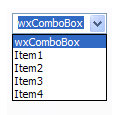
\includegraphics[width=119px]{pp_07}
    \caption{wxComboBox}
\end{figure}

We developed a small prototype just to get an experience of how it could look like and to check if the functionality works as planned. Even though everything worked fine we still had some issues concerning the appearance.
While it looks a lot like we wanted the suggestion panel to look it still has some major points that had to be criticised. Firstly, there is an arrow which shows or hides the panel on click. We did not have the intention of letting the user take this action because our focus was on making the recommendation windows as useful as possible so that it is only there when the user could need it but at the same time does not bother him if he does not need it. If the user had to hide the panel, the basic principle of this module would be broken. Secondly, many of the predefined window styles are restricted to a specific operating system. Due to the fact that we wanted OctoTagger to be as cross platform compatible as possible this was an extremely strong point of criticism. Both of these issues brought us to the point of saying that a wxCombobox is no adequate solution.

\subsubsection{Solution}
While looking in the internet for other possible options we stumbled upon an open source module, named \emph{wxautocompletectrl} \cite{autocomplete},which is free to use for everybody. It seemed to fit our needs extremely well so we took a closer look at it. Since many of the things we needed the module to do were already implemented, we only had to create, rewrite and delete a few functions to complete it. 

The module consists of two classes, one being \textit{Suggestion-Popup} and the other one being \textit{AutocompleteTextCtrl}. As for the first one the user has to specify the target frame as an argument. It creates the popup window containing the suggestions, which is a \textit{wxHtmlListBox}, and also defines the event handlers for tag selections. The latter class handles the tagging process when a suggested tag is clicked on or pressed via the \textit{ENTER} key. Furthermore, it sets the suggestions based on a given array and filters them accordingly to what has been typed into the tag bar.
This is how the suggestion panel could look like when one or multiple files are selected and the user has not typed anything into the tag bar:

\begin{figure}[H]
    \centering
    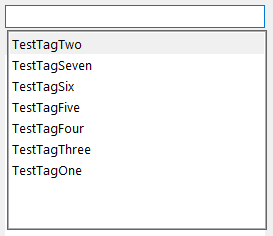
\includegraphics[width=200px]{pp_08}
    \caption{Suggestion panel without text typed in}
\end{figure}

Every tag is listed in the window, ordered by the frequency of how often a tag is used and the correlation of tags between the chosen files. If one types in text into the tag bar, the suggestions will be filtered appropriately to what has been typed in. After doing so the panel could look like this:

\begin{figure}[H]
    \centering
    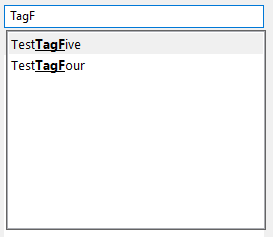
\includegraphics[width=200px]{pp_09}
    \caption{Suggestion panel with text typed in}
\end{figure}

It can be seen that the list is now styled, which is the reason for the used \textit{wxHtmlListBox} because the written text gets wrapped in <b> and <u> HTML-tags for better visibility.


